\documentclass[12pt]{article}

\usepackage{stickstootext}
\usepackage[stickstoo,vvarbb]{newtxmath}
\usepackage[scale=0.90]{tgheros}
\usepackage[scale=1]{inconsolata}
\usepackage{pst-pdf}
\usepackage{psfrag}
\usepackage{icomma}

\pagestyle{empty}

\begin{document}

\begin{psfrags}
    \psfrag{g}[c][c]{\small $G(s)$}
    \psfrag{c}[c][c]{\small $G_C(s)$}
    \psfrag{r}[c][c]{\footnotesize $R(s)$}
    \psfrag{y}[c][c]{\footnotesize $Y(s)$}
    \psfrag{e}[c][c]{\footnotesize $E(s)$}
    \psfrag{u}[c][c]{\footnotesize $U(s)$}
    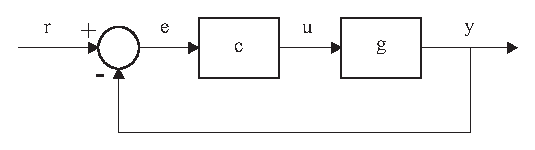
\includegraphics[scale=1,trim={0pt 0pt 0pt 0pt}]{blockdiagram.eps}
    % trim pode aumentar ou diminuiur as margens da figura
\end{psfrags}

\end{document}